\documentclass{tufte-book}\usepackage[]{graphicx}\usepackage[]{color}
%% maxwidth is the original width if it is less than linewidth
%% otherwise use linewidth (to make sure the graphics do not exceed the margin)
\makeatletter
\def\maxwidth{ %
  \ifdim\Gin@nat@width>\linewidth
    \linewidth
  \else
    \Gin@nat@width
  \fi
}
\makeatother

\usepackage{Sweavel}


\usepackage[flexible]{optional}
\usepackage{tufte-larger}
\usepackage[some]{background}
\usepackage{amssymb,amsmath}
\usepackage{amsmath, amssymb,txfonts,bm}
\usepackage{checkend}
\usepackage{nextpage}
\usepackage{listings}
\usepackage{framed}
\usepackage{float}
\usepackage{colortbl}
\usepackage{cprotect}
\usepackage{enumitem}
\usepackage{makeidx}
\makeindex
\usepackage{index}
\usepackage{multicol}
\newindex{fun}{fdx}{fnd}{Index of R Symbols and Functions}

% \newenvironment{knitrout}{\setlength{\topsep}{0mm}}{}
% \newcommand{\flexicol}{fullflexible}
\newcommand{\flexicol}{fixed}

\lstdefinestyle{Rstyle}{%
  fancyvrb=false,escapechar=`,language=R,%
  basicstyle={\Rcolor\Sweavesize\ttfamily},%         Added \ttfamily
  backgroundcolor=\Rbackground,%
  showstringspaces=false,%
  keywordstyle=\Rcolor,%
  commentstyle={\Rcommentcolor\ttfamily\itshape},%
  %literate=                                         Removed
  alsoother={$},%
  alsoletter={.<-},%
  otherkeywords={!,!=,~,$,*,\&,\%/\%,\%*\%,\%\%,<-,<<-,/},%
  escapeinside={(*}{*)}}%

\makeatletter
\renewenvironment{theindex}{%
  \columnseprule \z@
  \columnsep 35\p@
\begin{multicols}{3}[\chapter*{\indexname}][10\baselineskip]%
  \addcontentsline{toc}{chapter}{\indexname}%
  \setlength\parindent{0pt}\pagestyle{plain}\let\item\@idxitem}
{\end{multicols}}
\makeatother

\hypersetup{colorlinks}% uncomment this line if you prefer colored hyperlinks (e.g., for onscreen viewing)

%%
% Book metadata
\title{Learning R: Open Source (Free) System for Statistics and Much Else}
\author[]{J H Maindonald}
\publisher{}

%%
% If they're installed, use Bergamo and Chantilly from www.fontsite.com.
% They're clones of Bembo and Gill Sans, respectively.
%\IfFileExists{bergamo.sty}{\usepackage[osf]{bergamo}}{}% Bembo
%\IfFileExists{chantill.sty}{\usepackage{chantill}}{}% Gill Sans

%\usepackage{microtype}

%%
% For nicely typeset tabular material
\usepackage{booktabs}

%%
% For graphics / images
\usepackage{graphicx}
\setkeys{Gin}{width=\linewidth,totalheight=\textheight,keepaspectratio}
\graphicspath{{figs/}}

% The fancyvrb package lets us customize the formatting of verbatim
% environments.  We use a slightly smaller font.
\usepackage{relsize,fancyvrb}
\fvset{fontsize=\normalsize}

%%
% Prints argument within hanging parentheses (i.e., parentheses that take
% up no horizontal space).  Useful in tabular environments.
\newcommand{\hangp}[1]{\makebox[0pt][r]{(}#1\makebox[0pt][l]{)}}

%%
% Prints an asterisk that takes up no horizontal space.
% Useful in tabular environments.
\newcommand{\hangstar}{\makebox[0pt][l]{*}}

%%
% Prints a trailing space in a smart way.
\usepackage{xspace}

%%
% Some shortcuts for Tufte's book titles.  The lowercase commands will
% produce the initials of the book title in italics.  The all-caps commands
% will print out the full title of the book in italics.
\newcommand{\vdqi}{\textit{VDQI}\xspace}
\newcommand{\ei}{\textit{EI}\xspace}
\newcommand{\ve}{\textit{VE}\xspace}
\newcommand{\be}{\textit{BE}\xspace}
\newcommand{\VDQI}{\textit{The Visual Display of Quantitative Information}\xspace}
\newcommand{\EI}{\textit{Envisioning Information}\xspace}
\newcommand{\VE}{\textit{Visual Explanations}\xspace}
\newcommand{\BE}{\textit{Beautiful Evidence}\xspace}

\newcommand{\TL}{Tufte-\LaTeX\xspace}

% Prints the month name (e.g., January) and the year (e.g., 2008)
\newcommand{\monthyear}{%
  \ifcase\month\or January\or February\or March\or April\or May\or June\or
  July\or August\or September\or October\or November\or
  December\fi\space\number\year
}

\renewcommand{\maketitlepage}[0]{%
  \cleardoublepage%
  {%
  \sffamily%
  \begin{fullwidth}%
  \fontsize{18}{20}\selectfont\par\noindent\textcolor{darkgray}{{\thanklessauthor}}%
  \vspace{11.5pc}%
%  \fontsize{27}{30}\selectfont\par\noindent\textcolor{darkgray}{{\thanklesstitle}}%
  \fontsize{40}{45}\selectfont\par\noindent\textcolor{darkgray}{{\thanklesstitle}}%
  \vfill%
  \fontsize{14}{16}\selectfont\par\noindent\allcaps{\thanklesspublisher}%
  \end{fullwidth}%
  }
  \thispagestyle{empty}%
  \clearpage%
}


% Prints an epigraph and speaker in sans serif, all-caps type.
\newcommand{\openepigraph}[2]{%
  %\sffamily\fontsize{14}{16}\selectfont
  \begin{fullwidth}
  \sffamily\large
  \begin{doublespace}
  \noindent{#1}\\% epigraph
  \noindent{#2}% author
  \end{doublespace}
  \end{fullwidth}
}

% Inserts a blank page
\newcommand{\blankpage}{\newpage\hbox{}\thispagestyle{empty}\newpage}

\usepackage{units}

% Typesets the font size, leading, and measure in the form of 10/12x26 pc.
\newcommand{\measure}[3]{#1/#2$\times$\unit[#3]{pc}}

% Macros for typesetting the documentation
\newcommand{\hlred}[1]{\textcolor{Maroon}{#1}}% prints in red
\newcommand{\hangleft}[1]{\makebox[0pt][r]{#1}}
\newcommand{\hairsp}{\hspace{1pt}}% hair space
\newcommand{\hquad}{\hskip0.5em\relax}% half quad space
\newcommand{\TODO}{\textcolor{red}{\bf TODO!}\xspace}
\newcommand{\ie}{\textit{i.\hairsp{}e.}\xspace}
\newcommand{\eg}{\textit{e.\hairsp{}g.}\xspace}
\newcommand{\na}{\quad--}% used in tables for N/A cells
\providecommand{\XeLaTeX}{X\lower.5ex\hbox{\kern-0.15em\reflectbox{E}}\kern-0.1em\LaTeX}
\newcommand{\tXeLaTeX}{\XeLaTeX\index{XeLaTeX@\protect\XeLaTeX}}
% \index{\texttt{\textbackslash xyz}@\hangleft{\texttt{\textbackslash}}\texttt{xyz}}
\newcommand{\tuftebs}{\symbol{'134}}% a backslash in tt type in OT1/T1
\newcommand{\doccmdnoindex}[2][]{\texttt{\tuftebs#2}}% command name -- adds backslash automatically (and doesn't add cmd to the index)
\newcommand{\doccmddef}[2][]{%
  \hlred{\texttt{\tuftebs#2}}\label{cmd:#2}%
  \ifthenelse{\isempty{#1}}%
    {% add the command to the index
      \index{#2 command@\protect\hangleft{\texttt{\tuftebs}}\texttt{#2}}% command name
    }%
    {% add the command and package to the index
      \index{#2 command@\protect\hangleft{\texttt{\tuftebs}}\texttt{#2} (\texttt{#1} package)}% command name
      \index{#1 package@\texttt{#1} package}\index{packages!#1@\texttt{#1}}% package name
    }%
}% command name -- adds backslash automatically
\newcommand{\doccmd}[2][]{%
  \texttt{\tuftebs#2}%
  \ifthenelse{\isempty{#1}}%
    {% add the command to the index
      \index{#2 command@\protect\hangleft{\texttt{\tuftebs}}\texttt{#2}}% command name
    }%
    {% add the command and package to the index
      \index{#2 command@\protect\hangleft{\texttt{\tuftebs}}\texttt{#2} (\texttt{#1} package)}% command name
      \index{#1 package@\texttt{#1} package}\index{packages!#1@\texttt{#1}}% package name
    }%
}% command name -- adds backslash automatically
\newcommand{\docopt}[1]{\ensuremath{\langle}\textrm{\textit{#1}}\ensuremath{\rangle}}% optional command argument
\newcommand{\docarg}[1]{\textrm{\textit{#1}}}% (required) command argument
\newenvironment{docspec}{\begin{quotation}\ttfamily\parskip0pt\parindent0pt\ignorespaces}{\end{quotation}}% command specification environment
\newcommand{\docenv}[1]{\texttt{#1}\index{#1 environment@\texttt{#1} environment}\index{environments!#1@\texttt{#1}}}% environment name
\newcommand{\docenvdef}[1]{\hlred{\texttt{#1}}\label{env:#1}\index{#1 environment@\texttt{#1} environment}\index{environments!#1@\texttt{#1}}}% environment name
\newcommand{\docpkg}[1]{\texttt{#1}\index{#1 package@\texttt{#1} package}\index{packages!#1@\texttt{#1}}}% package name
\newcommand{\doccls}[1]{\texttt{#1}}% document class name
\newcommand{\docclsopt}[1]{\texttt{#1}\index{#1 class option@\texttt{#1} class option}\index{class options!#1@\texttt{#1}}}% document class option name
\newcommand{\docclsoptdef}[1]{\hlred{\texttt{#1}}\label{clsopt:#1}\index{#1 class option@\texttt{#1} class option}\index{class options!#1@\texttt{#1}}}% document class option name defined
\newcommand{\docmsg}[2]{\bigskip\begin{fullwidth}\noindent\ttfamily#1\end{fullwidth}\medskip\par\noindent#2}
\newcommand{\docfilehook}[2]{\texttt{#1}\index{file hooks!#2}\index{#1@\texttt{#1}}}
\newcommand{\doccounter}[1]{\texttt{#1}\index{#1 counter@\texttt{#1} counter}}

% Generates the index
% \usepackage{makeidx}

% \definecolor{fgcolor}{rgb}{0.345, 0.345, 0.345}
\definecolor{light}{gray}{.9}
\definecolor{gray40}{gray}{.4}
\definecolor{gray80}{gray}{.8}
\definecolor{gray90}{gray}{.9}

\newcommand{\txtt}[1]{\texttt{#1}}
\newcommand{\margtt}[1]{{\footnotesize \texttt{#1}}}

 \lstnewenvironment{verbcode}
 {\lstset{language=R, xleftmargin=4pt, frame=single, framerule=0pt,
          basicstyle=\small\ttfamily,
         columns=\flexicol,
          showstringspaces=false, backgroundcolor=\color{light}}}
 {}

\newenvironment{itemizz}%
  {\begin{itemize} %
    \setlength{\itemsep}{2pt}%
    \setlength{\parskip}{2pt}} %
  {\end{itemize}}

\begin{document}
% Front matter
\frontmatter




%

\setsidenotefont{\small}
\setcaptionfont{\small}
\setmarginnotefont{\small}
% \setcitationfont

\SetBgContents{
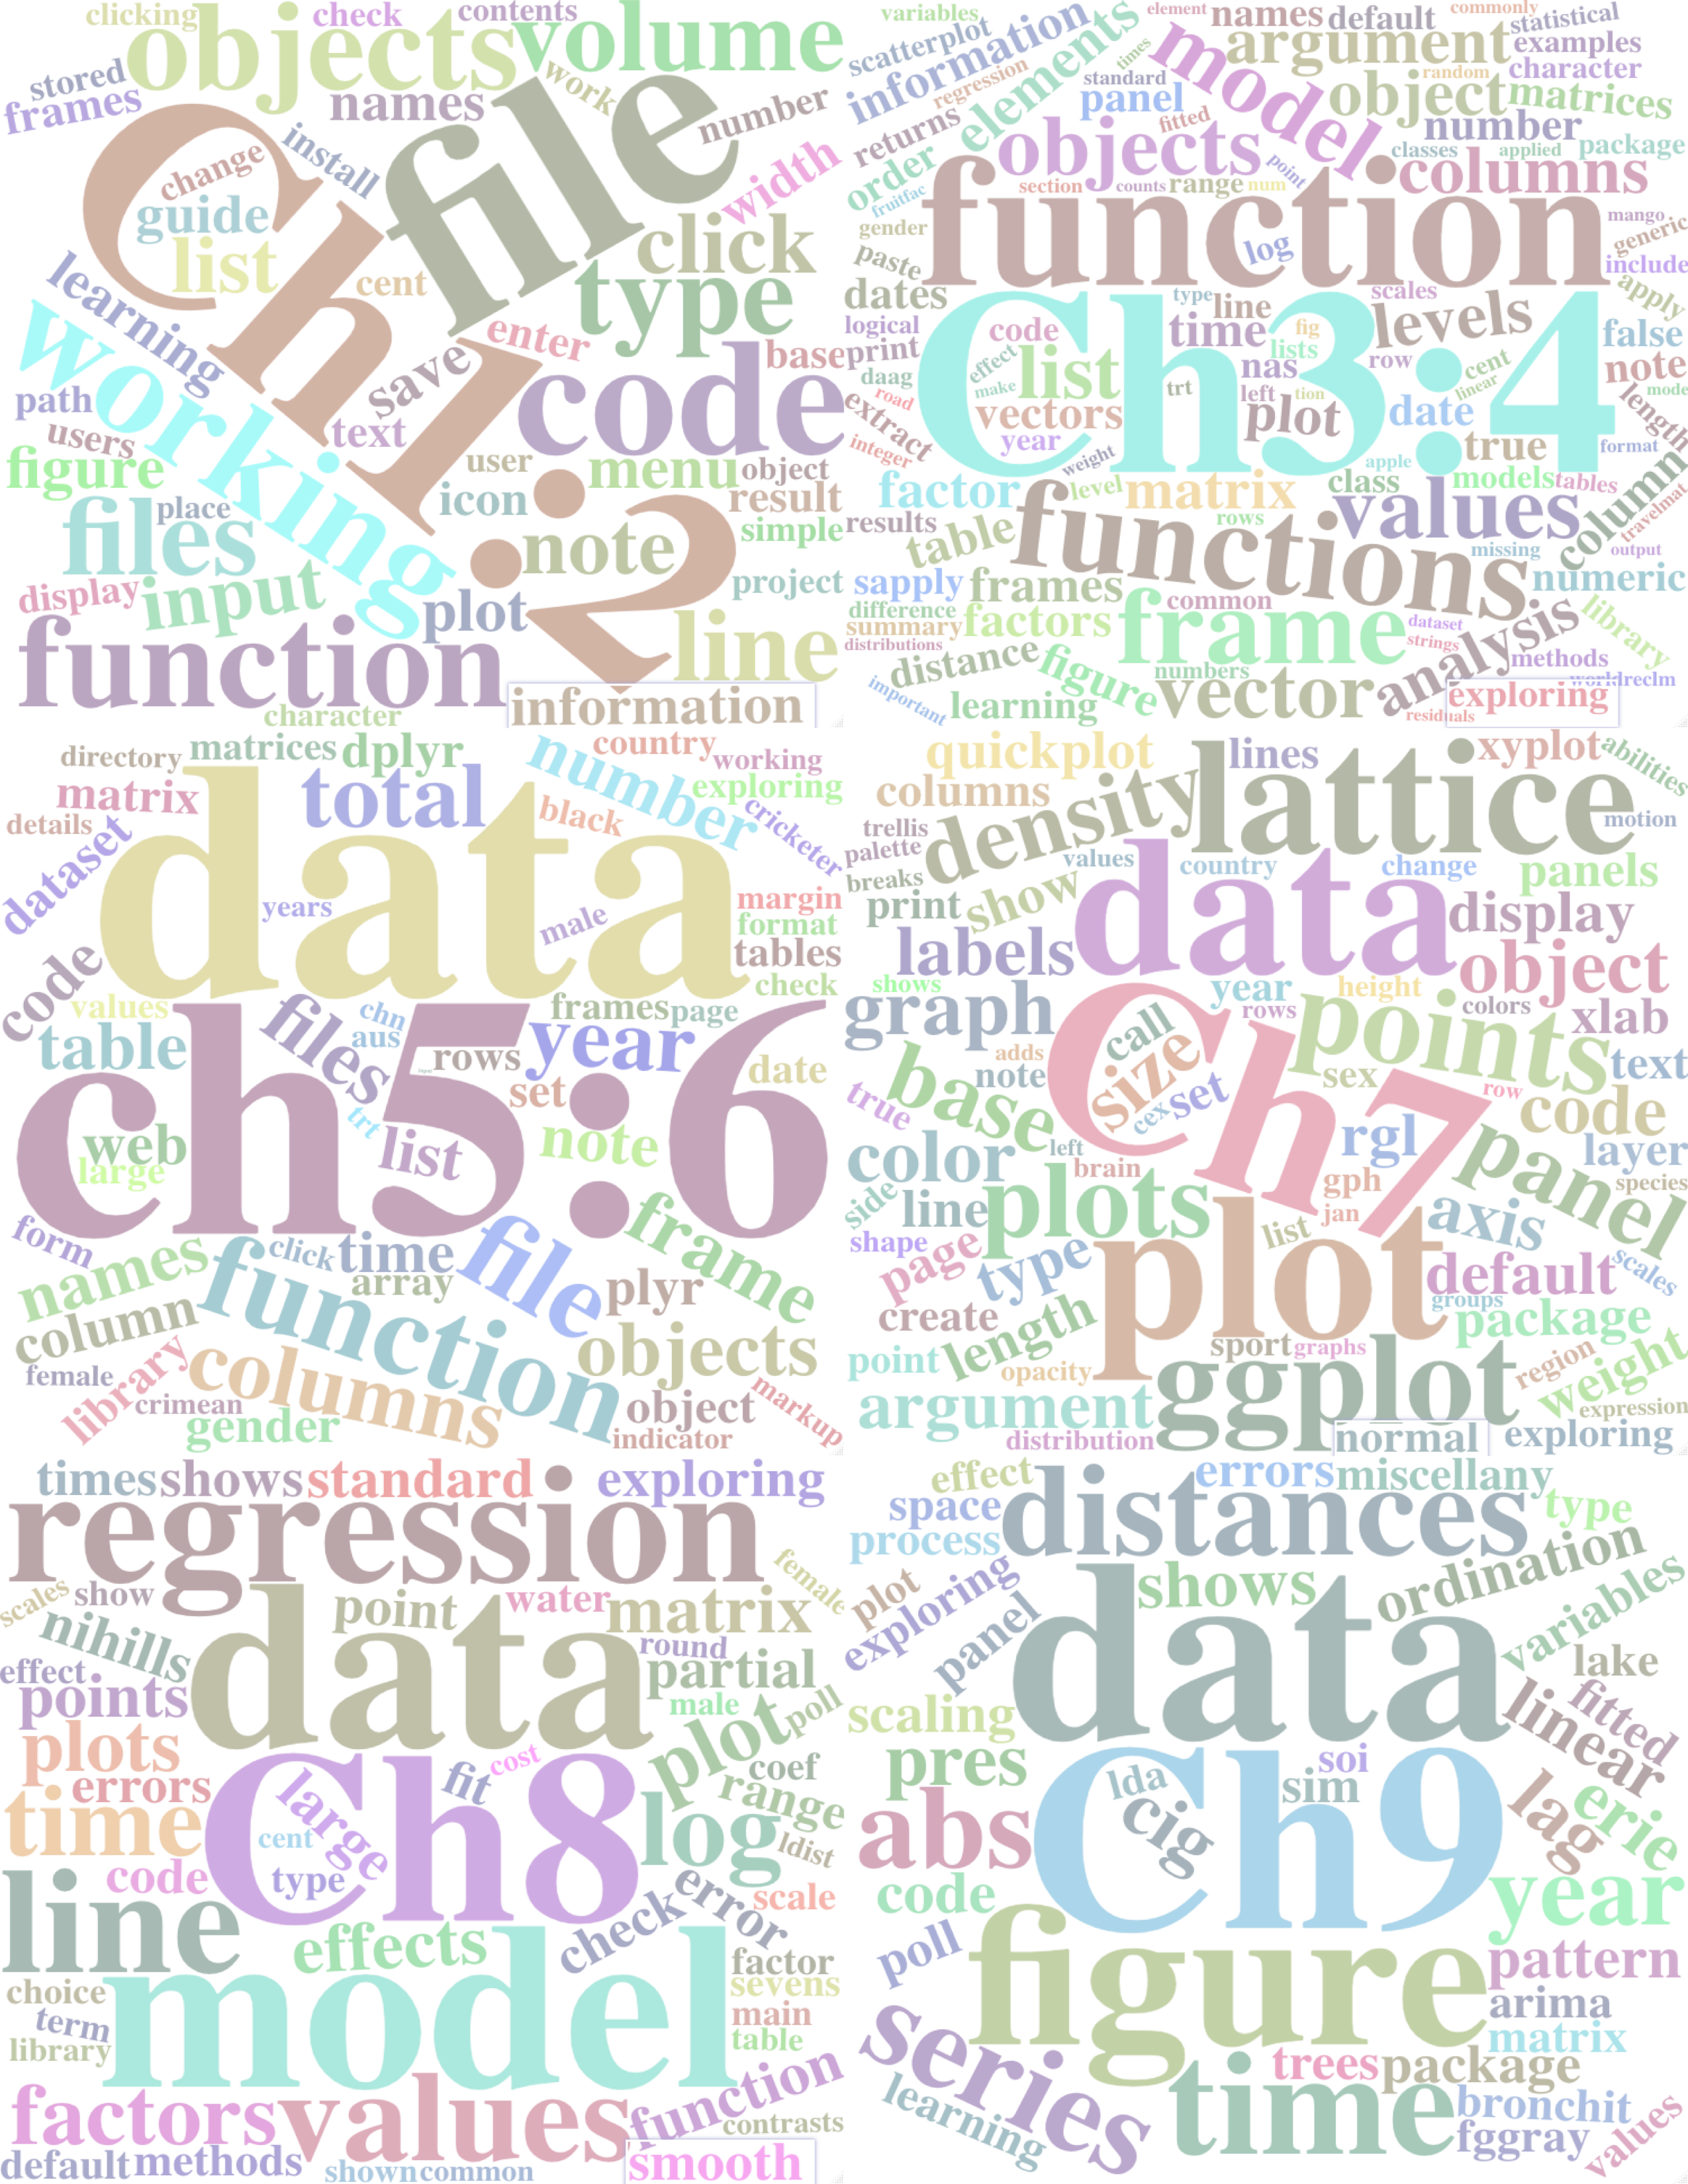
\includegraphics{figs-inc/cover-bg.pdf}
}
\SetBgScale{3.5}
\SetBgColor{gray!70}
\SetBgOpacity{0.2}
\BgThispage
\bmdefine\bX{\mathbf{X}}
\bmdefine\bP{\mathbf{P}}
\bmdefine\sfX{\bm{\textsf{\textmd{X}}}}
% \pagestyle{headings}

% r.1 blank page
% \blankpage

% v.2 epigraphs
% r.3 full title page
\maketitle

% v.4 copyright page
\newpage
\begin{fullwidth}
~\vfill
\thispagestyle{empty}
\setlength{\parindent}{0pt}
\setlength{\parskip}{\baselineskip}
Copyright \copyright\ \the\year\ \thanklessauthor\\
Copies may be made for individual study and research.  Other uses
are prohibited.

% \par\smallcaps{Published by \thanklesspublisher}

% \par\smallcaps{tufte-latex.googlecode.com}

\par\textit{\monthyear}
\end{fullwidth}
\vfill

\thispagestyle{empty}
\openepigraph{%
S has forever altered the way people analyze, visualize, and
manipulate data... S is an elegant, widely accepted, and enduring
software system, with conceptual integrity, thanks to the insight,
taste, and effort of John Chambers.
}{{\itshape From the citation for the 1998 Association for Computing Machinery
Software award.}
}
\vfill
\openepigraph{%
A big computer, a complex algorithm and a long time does not equal
science.
}{Robert Gentleman}
\vfill


%
% r.5 contents
\tableofcontents


% \begin{fullwidth}
% \listoffigures
% \end{fullwidth}

% \listoftables

% r.7 dedication
% \cleardoublepage
% ~\vfill
% \begin{doublespace}
% \noindent\fontsize{18}{22}\selectfont\itshape
% \nohyphenation
% Dedicated to the creators of S and R.
% \end{doublespace}
% \vfill
% \vfill

% r.9 introduction
\cleardoublepage
\chapter*{Introduction}

% !Rnw root = learnR.Rnw




\section*{The scope of these notes}

These notes were developed over the course of more than a
decade, for use in R courses that were presented to groups
within universities, within CSIRO, and within Government
departments.  Each new course offered the chance to 
extend and refine the content, and to add content that
was tuned to the requirements of the new audience.  
The result is a somewhat eclectic mix of material.
The notes are provided here with the intention that
others will be free to add to them, or to develop them
for their own purposes.
%
%
\section*{Commentary on R}

\subsection*{General}
R has extensive \marginnote{R is free to download from a CRAN site
  (see above).  It runs on all common types of system -- Windows, Mac,
  Unix and Linux.}  graphical abilities that are tightly linked with
its analytic abilities. A new release of base R, on which everything
else is built appears every few months.

The major part of R's abilities for statistical analysis
and for specialist graphics comes from the extensive enhancements that
the packages build on top of the base system.  Its abilities are
further extended by an extensive range of interfaces into
other systems\sidenote{These include Python, SQL and other
  databases, parallel computing using MPI, and Excel.}

The main part of the R system -- base R plus the recommended packages
-- is under continuing development.

\subsection*{The R user base}

Statistical and allied professionals\marginnote{ The R Task Views web
  page (\url{http://cran.csiro.au/web/views/}) notes, for application
  areas where R is widely used, relevant packages.} have found R
  especially attractive, both for the access that it gives to
  cutting edge tools, and as a platform for developing new tools.
Additionally, the R system has found wide use among working
scientists whose data analysis requirements justify the time
needed to gain the necessary R skills.  It is finding use, also, as
an environment in which to embed applications whose primary focus
is not data analysis or graphics.


\subsection*{Getting help}

\begin{fullwidth}
\fbox{\parbox{1.15\textwidth}{
{\bf Note the web sites:}\\[4pt]
Wikipedia:\newline
\url{http://en.wikipedia.org/wiki/R_(programming_language)}\\[3pt]
R-downunder (low traffic, friendly):\newline
\url{http://www.stat.auckland.ac.nz/mailman/listinfo/r-downunder}\\[3pt]
Stackoverflow\newline
\url{http://stackoverflow.com/questions/tagged/r}.
}}
\end{fullwidth}
\vspace*{8pt}

The r-help mailing list\marginnote{Details of this and other lists can
  be found at: \url{http://www.r-project.org}. Be sure to check the
  available documentation before posting to r-help. List archives can
  be searched for previous questions and answers.}  serves, especially
for users with a technical bent, as an informal support network.  The
R community expects users to want more than a quick cook-book fix, and
to show a willingness to work at improving statistical knowledge.

Novices will find the low traffic R-downunder list more friendly and
helpful than the main R mailing list. Its subscribers include some
highly expert individuals.

\subsection*{Important R web links}

\marginnote{CRAN is the primary R `repository'.  Among
  package repositories that supplement CRAN, note in
  particular the Bioconductor repository
  (\url{http://www.bioconductor.org}), which caters for
  high throughput genomic data.}
\noindent
\fbox{\parbox{\textwidth}{
{\bf Note the following web sites:}\\[4pt]
CRAN (Comprehensive R Archive Network):\newline
\url{http://cran.r-project.org}\\[3pt]
Obtain R and R packages from a CRAN mirror in the local region.
An Australian mirror (one of two) is: \url{https://cran.csiro.au/}\\[3pt]
For New Zealand, use \url{http://cran.stat.auckland.ac.nz}\\
R homepage: \url{https://www.r-project.org/}\\[3pt]

For various useful links click, from an R session that uses the
GUI, on the menu item \underline{R help}. Then, on the browser window
that pops up, look under \underline{Resources}}}



\subsection*{The origins and future of R}

The R system implements a dialect of the S language \marginnote{Open
  source systems that might have been the basis for an R-like project
  include Scilab, Octave, Gauss, Lisp-Stat, Python, and now Julia.
  None of these match the range and depth of R's packages.  
  Julia, which strongly outperforms R in execution time comparisons
 that appear on the Julia website \url{http://julialang.org},
 has not had time to establish a clear place for itself.}
that was developed at AT\&T Bell Laboratories as a general purpose
scientific language, with especial strengths in data manipulation,
graphical presentation and statistical analysis. The commercial
S-PLUS implementation popularized the S language, giving a user
base into which R could tap.

Ross Ihaka and Robert Gentleman, both at that time from the University
of Auckland, developed the initial version of R, for use in teaching.
Since mid-1997, development has been overseen by a `core team'
of about a dozen people, drawn from different institutions worldwide.

\marginnote[12pt]{More than 12,000 packages are, as of January 2018,
available through the CRAN sites.}
With the release of version 1.0 in early 2000, R became a serious tool
for professional use.  Since 2004, the number of packages has
increased at a rate of slightly more than 25\% per annum.

\marginnote[12pt]{R code looks at first glance like C code. The R
interpreter is modeled on the Scheme LISP dialect.}
The R system uses a language model that dates from the 1980s.
Any change to a more modern language model is likely to be
evolutionary.  Details of the underlying computer implementation
are in a process of limited continual change. 

  \subsection*{Interactive development environments -- editors and more}
  \marginnote{Note also Emacs, with the ESS (Emacs Speaks Statistics)
    addon. is This is a feature-rich environment that can be daunting
    for novices.  It runs on Windows as well as Linux/Unix and Mac.
    Note also, for Windows, the Tinn-R editor
    (\url{http://www.sciviews.org/Tinn-R/}).}  RStudio
  (\url{http://rstudio.org/}) is a very attractive run-time
  environment for R, available for Windows, Mac and Linux/Unix
  systems.  This has extensive abilities for managing projects, and
  for working with code.  It is a highly recommended alternative to
  the GUIs that come with the Windows and Mac OS X binaries that are
  available from CRAN sites.

\subsection*{Pervasive unifying ideas}
Ideas that pervade R include:\\[-8pt]
\marginnote{Expressions can be:\\
\vspace*{-8pt}
\begin{list}{}{\setlength{\itemsep}{2pt} \setlength{\parsep}{0pt}}
\item[] evaluated (of course)

\item[] printed on a graph (come to think of it, why not?)
\end{list}

\noindent There are many unifying computational features.  Thus
any `linear' model (lm, lme, etc) can use spline basis
  functions to fit spline terms.
}
\begin{list}{}{\setlength{\itemsep}{1pt} \setlength{\parsep}{1pt}}
\item[] Generic functions for common tasks -- print, summary, plot, etc.
(the Object-oriented idea; do what that ``class'' of object requires)

\item[] Formulae, for specifying graphs, models and tables.

\item[] Language structures can be manipulated, just like any
data object (Manipulate formulae, expressions, function argument
lists, \dots)

\item[] Lattice (trellis) and ggplot graphics offer innovative
  features that are widely used in R packages.  They aid the provision
  of graphs that reflect important aspects of data structure.

\end{list}
Note however that these are not uniformly implemented through R.
This reflects the incremental manner in which R has developed.

\subsection*{Data set size}
R's evolving technical design has allowed it,\marginnote{An important
  step was the move, with the release of version 1.2, to a dynamic
  memory model.} taking advantage of advances in computing hardware,
to steadily improve its handling of large data sets. The flexibility
of R's memory model does however have a cost\sidenote{The difference
  in cost may be small or non-existent for systems that have a 64-bit
  address space.} for some large computations, relative to systems
that process data from file to file.

\subsection*{Good planning,  informed analysis and reliable software}

While the R system
\marginnote{Take particular care with newer or little-used abilities
in contributed packages.  These may not have been much tested,
unless by their developers.} is unique in the extent of close
scrutiny that it receives from highly expert users, the same
warnings apply as to any statistical system.  The base system and
the recommended packages get unusually careful scrutiny.

  The scientific context, has crucial implications for the experiments
  that it is useful to do, and for the analyses that are meaningful.
  Available statistical methodology, and statistical and computing
  software and hardware, bring their own constraints and opportunities.

\textit{Statistics of data collection}\marginnote{Always, one
has to ask whether data are available, or can be collected, 
that allow the required inferences.} encompasses statistical
\textit{experimental design}, sampling design, and data collection
more generally. Subject area insights can be crucial. 

Once the data have been collected, the challenges are then those of
data analysis and of interpretation and presentation of results. 
Effective data analysis must take account of the limitations
inherent in the data, an understanding of the statistical issues,
and 
risks that arise from inadequate understanding of the statistical
issues.
For
this, software that is of high quality must be complemented with the
critical resources of well-trained and well-informed minds.

\section*{Documentation and Learning Aids}
\paragraph{R podcasts:} See for example
\url{http://www.r-podcast.org/}

\paragraph{Official Documentation:}
Users who are working through these notes on their own should
have available for reference the document
``An Introduction to R'', written by the R Development Core Team.
To download an up-to-date copy, go to CRAN.

\paragraph{Web-based Documentation:}

Go to \url{http://www.r-project.org}\marginnote{Also
  \url{http://wiki.r-project.org/rwiki/doku.php}}
and look under \underline{Documentation}.
There are further useful links under \underline{Other}.

\paragraph{The R Journal (formerly R News):}
Successive issues are a mine of useful information.
These can be copied down from a CRAN site.

\paragraph{Books:}
See \url{http://www.R-project.org/doc/bib/R.bib} for a list of
R-related books that is updated regularly. Here, note
especially:\\[3pt]
\noindent
Maindonald, J. H. \& Braun, J. H. 2010. Data Analysis \&
  Graphics Using R. An Example-Based Approach. 3$^{rd}$ edn, Cambridge
  University Press,
  Cambridge, UK, 2010.\\
\noindent
\url{http://www.maths.anu.edu.au/~johnm/r-book.html}

\cleardoublepage
\section*{Notes for Readers of this Text}

\subsection*{Asterisked Sections or Subsections}

Asterisks are used to identify material that is more technical or
specialized, and that might be omitted at a first reading.

\subsection*{The {\em DAAGviz} package}
\marginnote{Note that {\em DAAGviz} is not available on CRAN.
It collects scripts and datasets together in a way that may be
useful to course participants.  Those materials are also
available separately.}
This package is an optional companion to these notes. To
download installation files (Windows, Mac or Linux) go to
the web page \url{https://www.acspri.org.au/springprogram2015},
navigate to the website for this course, and log in with
your ACSPRI user name and password.  A link will appear
at the bottom of the page, under {\bf Files for this course}.
Alternatively, go the web address \url{https://www.acspri.org.au/node/1566} and log in.

\begin{marginfigure}Assuming that the {\em DAAGviz} package has been installed, it can be attached thus:
\begin{Schunk}
\begin{Sinput}
library(DAAGviz)
\end{Sinput}
\end{Schunk}
\end{marginfigure}
Once attached, this package gives access to:
\begin{itemizz}
\item[-]
\begin{marginfigure}[78pt]
More succinctly, use the function \margtt{getScript()}:\\[-3pt]
\begin{Schunk}
\begin{Sinput}
## Place Ch 5 script in
## working directory
getScript(5)
\end{Sinput}
\end{Schunk}
\end{marginfigure}
Scripts that include all the code. To access these scripts do, e.g.
\begin{Schunk}
\begin{Sinput}
## Check available scripts
dir(system.file('scripts', package='DAAGviz'))
## Show chapter 5 script
script5 <- system.file('scripts/5examples-code.R',
                        package='DAAGviz')
file.show(script5)
\end{Sinput}
\end{Schunk}
\item[-]
\begin{marginfigure}[24pt]
More succinctly, use the function \margtt{sourceFigFuns()}:\\[-3pt]
\begin{Schunk}
\begin{Sinput}
## Load Ch 5 functions
## into workspace
sourceFigFuns(5)
\end{Sinput}
\end{Schunk}
\end{marginfigure}
Source files (also scripts) for functions that can be used to
  reproduce the graphs. These are available for Chapters 5 to 15
only.  To load the Chapter 5 functions into the workspace,
use the command:
\begin{Schunk}
\begin{Sinput}
path2figs5 <- system.file('doc/figs5.R',
                          package='DAAGviz')
source(path2figs5)
\end{Sinput}
\end{Schunk}
\item[-] The datasets \txtt{bronchit}, \txtt{eyeAmp}, and
  \txtt{Crimean}, which feature later in these notes.
\end{itemizz}
\newpage

\subsection*{Alternative sources for some datasets}
{\color{gray40}
The web page \url{http://maths-people.anu.edu.au/~johnm/} may in a few cases
be a convenient source for datasets that are referred to in this text:
\begin{itemizz}
\item[-] 
Look in \url{http://maths-people.anu.edu.au/~johnm/r/rda} for
  various image ({\bf .RData}) files.\sidenote{{\em Image} files hold 
  copies of one or more R objects, in a format that facilitates rapid 
  access from R.}  Use the function \txtt{load()} to bring any of these 
  into R.
\item[-] Look in \url{http://maths-people.anu.edu.au/~johnm/datasets/text}
  for the files {\bf bestTimes.txt}, {\bf molclock.txt}, and other such
  text files.
\item[=] Look in \url{http://maths-people.anu.edu.au/~johnm/datasets/csv}
  for several {\bf .csv} files.
\end{itemizz}
\vspace*{-9pt}
}


% Start the main matter (normal chapters)
\mainmatter
\setcounter{secnumdepth}{2}

\chapter{Preliminaries}

% !Rnw root = learnR.Rnw




\section{Installation of R}

Click as indicated in the successive panels to download R for
Windows from the web page \url{http://cran.csiro.au}:
\vspace*{-3pt}

\begin{figure}
\fbox{
\includegraphics{figs-inc/01i-cran.jpg}
}
\vspace*{2pt}

\fbox{
\includegraphics{figs-inc/01i-base.jpg}
}
\vspace*{2pt}

\fbox{
\includegraphics{figs-inc/01i-download.jpg}
}
\caption{This shows a sequence of clicks that will download
  the R installation file from \url{cran.csiro.edu}. At the time of writing,
  the website will offer R-3.4.3 rather than R-2.13.0. The site
  \url{cran.csiro.edu} is one of two Australian CRAN (Comprehensive R Archive
  Network) sites. The other is:
  \url{http://cran.ms.unimelb.edu.au/}}
\end{figure}

\begin{marginfigure}
\begin{center}
\begin{minipage}[c]{0.8\textwidth}
\includegraphics{figs-inc/01i-icons.jpg}
\end{minipage}
\end{center}
\caption{On 64-bit Windows systems the default installation
process creates two icons, one for 32-bit R and one for 64-bit R.
Additional icons can be created as desired.
}
\end{marginfigure}

Click on the downloaded file to start installation.  Most users will
want to accept the defaults.  The effect is to install the R base
system, plus recommended packages, with a standard ``off-the-shelf''
setup.  Windows users will find that one or more desktop R icons have
been created as part of the installation process.

Depending on the intended tasks, it may be necessary to install
further packages. Section \ref{sec:pkgs} describes alternative
ways to install packages.

An optional additional step is to install RStudio.
\marginnote{Clicking on the RStudio icon to start a session will at
  the same time start R. RStudio has its own command line interface,
  where users can type R commands.}  RStudio has abilities that
help in managing workflow, in navigating between projects, and in
accessing R system information.  See Chapter \ref{ch:rstudio}.

\section{First steps}\label{sec:step1}

\marginnote{Readers who have RStudio running can type their commands
in the RStudio command line panel.}
Click on an R icon to start an R session.  This opens an R command
window, prints information about the installed version of R, and
gives a command prompt.

\begin{figure}
\includegraphics[trim=0 18 0 0]{figs-inc/01i-gui.jpg}
\caption{Windows command window at startup. This shows the default MDI
  (multiple display) interface. For running R from the R Commander,
  the alternative SDI (single display) interface may be required, or
  may be preferable.  The Mac GUI has a SDI type interface; there is
  no other option.}
\end{figure}

\noindent
The \texttt{$>$} prompt that appears on the final line
is an invitation to start typing R commands:

Thus, type \txtt{2+5} and press the Enter key.
The display shows:
\begin{Schunk}
\begin{Sinput}
> 2+5
\end{Sinput}
\begin{Soutput}
[1] 7
\end{Soutput}
\end{Schunk}
\noindent
\marginnote[-1.0cm]{The \margtt{[1]} says, a little strangely, ``first
  requested element will follow''. Here, there is just one element.}
The result is 7. The output is immediately followed by the \txtt{>}
prompt, indicating that R is ready for another command.

Try also:
\marginnote[48pt]{Typing \margtt{result} on the
command line has printed the value 7.}
\begin{Schunk}
\begin{Sinput}
> result <- 2+5
> result
\end{Sinput}
\begin{Soutput}
[1] 7
\end{Soutput}
\end{Schunk}

\marginnote[7pt]{Technically, the \textit{workspace} is one of a
  number of \textit{databases} where objects may be stored.}
The object \margtt{result} is stored in the \textit{workspace}.
The {\em workspace} holds objects that the user has created or input,
or that were there at the start of the session and not later removed

Type \txtt{ls()} to list the objects in the workspace, thus:
\begin{Schunk}
\begin{Sinput}
> ls()
\end{Sinput}
\begin{Soutput}
[1] "result"
\end{Soutput}
\end{Schunk}
\marginnote[-24pt]{The object \margtt{result} was added to
a previously empty workspace.}

Figure \ref{fig:cmds} shows, with annotations, the screen as
it appears following the above sequence of commands.

\begin{figure}
\includegraphics{figs-inc/01i-cmds.jpg}
\caption{This shows the sequence of commands that are demonstrated in
  the text, as they appear on the screen, with added
  annotation.\label{fig:cmds}}
\end{figure}

An R session is structured as a hierarchy of databases. Functions that
were used or referred to above --- such as \txtt{ls()} -- are from a
database or {\em package} that is part of the R system.  Objects that
the user has created or input, or that were there at the start of the
session and not later removed, are stored in the {\em workspace}.

\marginnote[12pt]{Technically, the R system refers to the workspace
as \txtt{.Globalenv}.}
The workspace is the user's database for the duration of a session.
It is a volatile database, i.e., it will disappear if not explicitly
saved prior to or at the end of the session.

\subsection{Points to note}
\noindent
\fbox{\parbox{\textwidth}{\vspace*{-9pt}
\begin{tabbing}
Demonstrations\= \txtt{example(plot)} x\= \kill
Printing \> Typing the name of an object (and pressing \underline{Enter})\\
\> displays (prints) its contents.\\[4pt]
Quitting \> To quit, type \txtt{q()}, (not \txtt{q})\\[4pt]
Case matters \> \txtt{volume} is different from \txtt{Volume}
% Examples \> To run examples from a help page, type, e.g.\\
%  \> \txtt{example(plot)} \> \txtt{\# Example from help(plot)}\\[4pt]
\end{tabbing}
\vspace*{-9pt}
}}
\vspace*{9pt}

Typing the name of an object (and pressing the \underline{Enter} key)
causes the printing of its contents, as above when \txtt{result} was
typed.  This applies to functions also. Thus type \txtt{q()} in order
to quit, not \txtt{q}.\footnote{Typing \txtt{q} lists the code for the
  function.}  One types \txtt{q()} because this causes the function
\txtt{q} to spring into action.

Upon typing \txtt{q()} and pressing the Enter key, a message will ask
whether to save the workspace image.\sidenote{Such an {\em image}
allows reconstruction of the workspace of which it forms an image!}
Clicking Yes (usually the safest
option) will save the objects that remain in the workspace -- any that
were there at the start of the session (unless removed or overwritten)
and any that have been added since.  The workspace that has been thus
saved is automatically reloaded when an R session is restarted in the
working directory to which it was saved.

\begin{figure}
\includegraphics{figs-inc/01i-cmds1.jpg}
\caption{Note the use of the special characters: \txtt{;} to separate
  multiple commands on the one line, \txtt{+} (generated by the
  system) to denote continuation from previous line, and \txtt{\#} to
  introduce comment that extends to end of line.\label{fig:cmds1}}
\end{figure}

Note that for names of R objects or commands, case is significant.
Thus \txtt{Myr} (millions of years, perhaps) differs from \txtt{myr}.
For file names,\sidenote[][-28pt]{Under Windows case
is ignored. For Unix case does distinguish.
(Mac OS X Unix is a partial exception.)} the operating system
conventions apply.

Commands may, as demonstrated in Figure \ref{fig:cmds1}, continue over
more than one line. By default, the continuation prompt is \txtt{+}.
As with the \txtt{>} prompt, this is generated by R, and appears on
the left margin.  Including it when code is entered will give an
error!  \marginnote[-30pt]{Here is a command that extends over two lines:\\
  \margtt{> result <-}\\
  \margtt{+ 2+5} }

\subsection{Some further comments on functions in R}

\marginnote{R is a functional language. Whenever a command is entered,
  this causes a function to run. Addition is implemented as a
  function, as are other such operations.} Common functions that users
  should quickly get to know include \margtt{print()}, \margtt{plot()}
  and \margtt{help()}.  Above, we noted the function \txtt{q()}, used
  to quit from an R session.

Consider the function \txtt{print()}. One can explicitly invoke it to print the
number 2 thus:
\begin{Schunk}
\begin{Sinput}
print(2)
\end{Sinput}
\begin{Soutput}
[1] 2
\end{Soutput}
\end{Schunk}
Objects on which the function will act are placed inside the round
brackets.  Such quantities are known as {\em arguments} to the function.

An alternative to typing \txtt{print(2)} is to
type \txtt{2} on the command line.  The function \txtt{print()}
is then invoked implicitly:
\begin{Schunk}
\begin{Sinput}
2
\end{Sinput}
\begin{Soutput}
[1] 2
\end{Soutput}
\end{Schunk}

\subsection{Help information}\label{ss:ch1-help}

Included on the information that appeared on the screen when R started
up, and shown in Figures \ref{fig:cmds} and \ref{fig:cmds1}, were brief
details on how to access R's built-in help information:
{\small
\begin{verbatim}
Type 'demo()' for some demos, 'help()' for on-line help, or
'help.start()' for an HTML browser interface to help.
\end{verbatim}
}
\noindent
The shorthand \txtt{?plot} is an alternative to typing
\txtt{help(plot)}.

Replace `\txtt{?}' by `\txtt{??}' for a wider search.  This invokes
the function \txtt{help.search()}, which looks for a partial match
in the title or concept fields as well as in the name.
\begin{marginfigure}[-15pt]
Examples of use of \txtt{??}:\\[-5pt]
\begin{Schunk}
\begin{Sinput}
??Arithmetic
??base::Arith
  # Search base R only
\end{Sinput}
\end{Schunk}
\end{marginfigure}

R has extensive built-in help information.  Be sure to check it out
as necessary.  Section \ref{sec:workinghelp} has further details on
what is available, beyond what you can get by using the help function.

\subsection{The working directory}\label{ss:workdir}

Associated with each session \marginnote{Under Windows, if R is
  started by clicking on an R icon, the working directory is that
  specified in the \underline{Start in} directory specified in the icon
  Preferences.  Subsection \ref{sec:fine-tune} has details on how to
specify the  \underline{Start in} directory for an icon.}
is a working directory where R will by default look
for files.  In particular:
\begin{itemize}
\item If a command inputs data from a file into the
workspace and the path is not specified, this is where R
will look for the file.
\item If a command outputs results to a file, and the path is not specified,
this is where R will place the file.
\item Upon quitting a session, the ``off-the-shelf'' setup will ask
  whether to save an ``image'' of the session. 
\marginnote{When R finds a {\bf .RData} file in the working
  directory at startup, that file will, in an off-the-shelf setup, 
  be used to restore the workspace.}
  Answering
  ``Yes'' has the result that the contents of the workspace are saved
  into a file, in the working directory, that has the name {\bf
    .RData}.  
\end{itemize}

For regular day to day use of R,
it is advisable to have a separate working
directory for each different project.
RStudio users will be asked to specify
a working directory when setting up a new ``project''.

\section{Installation of R Packages}\label{sec:pkgs}
\marginnote[10pt]{ A fresh install of R packages is typically required
  when moving to a new major release (e.g., from a 3.0 series release
  to a 3.1 series release).}

\noindent
\fbox{
  \parbox{\linewidth}{ \noindent
\textbf{Installation of R Packages (Windows \& MacOS X)} \\[3pt]
Start R (e.g., click on the R icon). Then use the relevant menu item to
install packages via an internet connection. This is (usually) easier than
downloading, then installing.\\[6pt]
For command line instructions to install packages, see below.
}}
\vspace*{6pt}

The functions that R provides are organised into packages.  The
packages that need to be installed, additional to those that come with
the initial ready-to-run system, will vary depending on individual
user requirements.  The GUIs --- MacOS X, Windows or Linux --- make
package installation relatively straightforward.

\subsection*{Installation of packages from the command line}

To install the R Commander from the command line, enter:
\marginnote{By default, a CRAN mirror is searched for the required
  package.  Refer back to the introduction for brief comments on
  CRAN.  Subsection \ref{ss:installpack} gives details of
  alternatives to CRAN. Note in particular the Bioconductor
  repository.}
\begin{Schunk}
\begin{Sinput}
install.packages("Rcmdr", dependencies=TRUE)
\end{Sinput}
\end{Schunk}
The R Commander has a number of dependencies, i.e., packages that
need to be installed for the R Commander to run.  Graphics packages
that are dependencies include \textit{rgl} (3D dynamic graphics),
\textit{scatterplot3d}, \textit{vcd} (visualization of categorical
data) and \textit{colorspace} (generation of color palettes, etc).

\subsection*{Installation of Bioconductor packages}
\marginnote[10pt]{For installation of Bioconductor packages from the GUI,
  see Subsection \ref{sec:repos}.}  To set your system up for use of
Bioconductor packages, type:
\begin{Schunk}
\begin{Sinput}
source("http://bioconductor.org/biocLite.R")
biocLite()
\end{Sinput}
\end{Schunk}
Additional packages can be installed thus:
\begin{Schunk}
\begin{Sinput}
biocLite(c("GenomicFeatures", "AnnotationDbi"))
\end{Sinput}
\end{Schunk}
See further \url{http://www.bioconductor.org/install/}.

\section{Summary}
\begin{itemizz}
\item[] One use of R is as a calculator, to evaluate arithmetic
expressions. Calculations can be carried out in parallel, across all
elements of a vector at once.

\item[] The R Commander GUI can be helpful in getting quickly into use
  of R for many standard purposes.  It may, depending on requirements,
  be limiting for serious use of R.

\item[] Use \txtt{q()} to quit from an R session. To retain objects in
  the workspace, accept the offer to save the workspace.
\end{itemizz}


\chapter{An Overview of R}\label{ch:oview}

% !Rnw root = learnR.Rnw




\marginnote{Read \margtt{c} as ``\underline{c}oncatenate'',
or perhaps as ``column''.\\[6pt]
\noindent Lists are widely used in R.  A data frame is a
special type of list,
used to collect together column objects under one name.}
\noindent
\fbox{\parbox{\textwidth}{\vspace*{-3pt}
\begin{tabular}{l}
{\bf Column Objects}\\
\qquad \txtt{width = c(11.3, 13.1, 20, 21.1, 25.8, 13.1)}\\[3pt]
\qquad \txtt{height = c(23.9, 18.7, 27.6, 28.5, 36, 23.4)}\\[4pt]
{\bf Data frame}\\
A data frame is a list of column objects, all of the same length.\\
\qquad \txtt{widheight <- data.frame( }\\
\qquad \qquad \txtt{width = c(11.3, 13.1, 20, 21.1, 25.8, 13.1),}\\
\qquad \qquad \txtt{height = c(23.9, 18.7, 27.6, 28.5, 36, 23.4)}\\
\qquad \txtt{ )}\\[4pt]
{\bf Also:} Arithmetic operations; simple plots; input of data.\\
\end{tabular}
\vspace*{-3pt}}}
\vspace*{3pt}

\section{Practice with R commands}
\marginnote{The R language has the standard abilities for evaluating
arithmetic and logical expressions.  There are numerous functions
that extend these basic arithmetic and logical abilities.}
Try the following
\begin{Schunk}
\begin{Sinput}
2+3        # Simple arithmetic
\end{Sinput}
\begin{Soutput}
[1] 5
\end{Soutput}
\begin{Sinput}
1:5        # The numbers 1, 2, 3, 4, 5
\end{Sinput}
\begin{Soutput}
[1] 1 2 3 4 5
\end{Soutput}
\begin{Sinput}
mean(1:5)  # Average of 1, 2, 3, 4, 5
\end{Sinput}
\begin{Soutput}
[1] 3
\end{Soutput}
\begin{Sinput}
sum(1:5)   # Sum of 1, 2, 3, 4, 5
\end{Sinput}
\begin{Soutput}
[1] 15
\end{Soutput}
\begin{Sinput}
(8:10)^2   # 8^2 (8 to the power of 2), 9^2, 10^2
\end{Sinput}
\begin{Soutput}
[1]  64  81 100
\end{Soutput}
\end{Schunk}

In addition to \txtt{log()}, note \txtt{log2()} and \txtt{log10()}:
\marginnote{A change by a factor of 2 is a one unit change
  on a log2 scale. A change by a factor of 10 is a one unit change
  on a log10 scale.}
\begin{Schunk}
\begin{Sinput}
log2(c(0.5, 1, 2, 4, 8))
\end{Sinput}
\begin{Soutput}
[1] -1  0  1  2  3
\end{Soutput}
\begin{Sinput}
log10(c(0.1, 1, 10, 100, 1000))
\end{Sinput}
\begin{Soutput}
[1] -1  0  1  2  3
\end{Soutput}
\end{Schunk}
\noindent
It turns out, surprisingly often, that logarithmic scales are
appropriate for one or other type of graph.  Logarithmic scales focus
on relative change --- by what factor has the value changed?

The following uses the relational operator \txtt{$>$}:
\marginnote{
Other relational operators are\\
\margtt{$<\quad >=\quad <\quad <=\quad ==\quad !=$}
}
\begin{Schunk}
\begin{Sinput}
(1:5) > 2  # Returns FALSE FALSE  TRUE  TRUE  TRUE
\end{Sinput}
\begin{Soutput}
[1] FALSE FALSE  TRUE  TRUE  TRUE
\end{Soutput}
\end{Schunk}

\subsection*{Demonstrations}

Demonstrations can be highly helpful in learning to use R's functions.
The following are some of demonstrations that are available for
graphics functions:
\begin{marginfigure}
Images and perspective plots:
\begin{Schunk}
\begin{Sinput}
demo(image)
demo(persp)
\end{Sinput}
\end{Schunk}
\end{marginfigure}
\begin{Schunk}
\begin{Sinput}
demo(graphics)   # Type <Enter> for each new graph
library(lattice)
demo(lattice)
\end{Sinput}
\end{Schunk}

\begin{marginfigure}For the following, the {\em vcd} package must be installed:
\begin{Schunk}
\begin{Sinput}
library(vcd)
demo(mosaic)
\end{Sinput}
\end{Schunk}
\end{marginfigure}

Especially for \txtt{demo(lattice)}, it pays to stretch the graphics
window to cover a substantial part of the screen.  Place the cursor on
the lower right corner of the graphics window, hold down the left
mouse button, and pull.

The following lists available demonstrations:
\begin{Schunk}
\begin{Sinput}
## List demonstrations in attached packages
demo()
## List demonstrations in all installed packages
demo(package = .packages(all.available = TRUE))
\end{Sinput}
\end{Schunk}

\section{A Short R Session}\label{ss:shortR}
We will work with the data set shown in Table
\ref{tab:travel}:

% latex table generated in R 3.0.1 by xtable 1.7-1 package
% Sat Jul 20 10:40:12 2013
\begin{table*}[ht]
\centering
\begin{tabular}{rrrrrrl}
  \hline
 & thickness & width & height & weight & volume & type \\
  \hline
Aird's Guide to Sydney & 1.30 & 11.30 & 23.90 & 250 & 351 & Guide \\
  Moon's Australia handbook & 3.90 & 13.10 & 18.70 & 840 & 955 & Guide \\
  Explore Australia Road Atlas & 1.20 & 20.00 & 27.60 & 550 & 662 & Roadmaps \\
  Australian Motoring Guide & 2.00 & 21.10 & 28.50 & 1360 & 1203 & Roadmaps \\
  Penguin Touring Atlas & 0.60 & 25.80 & 36.00 & 640 & 557 & Roadmaps \\
  Canberra - The Guide & 1.50 & 13.10 & 23.40 & 420 & 460 & Guide \\
   \hline
\end{tabular}
\vspace*{15pt}

\caption{Weights and volumes, for six Australian travel
books.}\label{tab:travel}
\end{table*}

\subsection*{Entry of columns of data from the command line}
The following enters data as numeric vectors:
\marginnote{Read \margtt{c} as
  ``\underline{c}oncatenate'', or perhaps as
  ``column''.  It joins elements together into a vector, here
  numeric vectors.}
\begin{Schunk}
\begin{Sinput}
volume <- c(351, 955, 662, 1203, 557, 460)
weight <- c(250, 840, 550, 1360, 640, 420)
\end{Sinput}
\end{Schunk}

Now store details of the books in the character vector \txtt{description}:
\marginnote{The end result is that objects \margtt{volume}, \margtt{weight}
and \margtt{description} are stored in the workspace.}
\begin{Schunk}
\begin{Sinput}
description <- c("Aird's Guide to Sydney",
 "Moon's Australia handbook",
 "Explore Australia Road Atlas",
 "Australian Motoring Guide",
 "Penguin Touring Atlas", "Canberra - The Guide")
\end{Sinput}
\end{Schunk}

\subsection*{Listing the workspace contents}

Use \txtt{ls()} to examine the current contents
of the workspace.
\begin{Schunk}
\begin{Sinput}
ls()
\end{Sinput}
\begin{Soutput}
[1] "description" "volume"      "weight"     
\end{Soutput}
\end{Schunk}
Use the argument \txtt{pattern} to specify a search pattern:
\begin{marginfigure}[40pt]
Note also:\\[-5pt]
\begin{Schunk}
\begin{Sinput}
ls(pattern="^des")
  ## begins with 'des'
ls(pattern="ion$")
  ## ends with 'ion'
\end{Sinput}
\end{Schunk}
\end{marginfigure}
\begin{Schunk}
\begin{Sinput}
ls(pattern="ume")   # Names that include "ume"
\end{Sinput}
\begin{Soutput}
[1] "volume"
\end{Soutput}
\end{Schunk}

\subsection*{Operations with numeric \txtt{vectors}}
Here are the values of \txtt{volume}
\begin{Schunk}
\begin{Sinput}
volume
\end{Sinput}
\begin{Soutput}
[1]  351  955  662 1203  557  460
\end{Soutput}
\end{Schunk}

To extract the final element of \txtt{volume}, do:
\begin{Schunk}
\begin{Sinput}
volume[6]
\end{Sinput}
\begin{Soutput}
[1] 460
\end{Soutput}
\end{Schunk}
For the ratio of weight to volume, i.e., the density, we can do:
\begin{Schunk}
\begin{Sinput}
weight/volume
\end{Sinput}
\begin{Soutput}
[1] 0.7123 0.8796 0.8308 1.1305 1.1490 0.9130
\end{Soutput}
\end{Schunk}

\subsection*{A note on functions}

For the \txtt{weight/volume} calculation, two decimal places in the output
is more than adequate accuracy. The following uses the function
\txtt{round()} to round to two decimal places:
\begin{marginfigure}[24pt]
More simply, type:
\begin{Schunk}
\begin{Sinput}
round(weight/volume, 2)
\end{Sinput}
\end{Schunk}
Providing the arguments are in the defined
order, they can as here be omitted from
the function call.
\end{marginfigure}
\begin{Schunk}
\begin{Sinput}
round(x=weight/volume, digits=2)
\end{Sinput}
\begin{Soutput}
[1] 0.71 0.88 0.83 1.13 1.15 0.91
\end{Soutput}
\end{Schunk}

\marginnote[11pt]{Many functions, among them \margtt{plot()} that is used
  for Figure \ref{fig:denplot}, accept unnamed as well as named
  arguments. The symbol `\margtt{\ldots}' is used to denote the possibility of
  unnamed arguments.}  Functions take {\em arguments} --- these supply
data on which they operate.  For \txtt{round()} the arguments are
`\txtt{x}' which is the quantity that is to be rounded, and
`\txtt{digits}' which is the number of decimal places that should
remain after rounding.

\marginnote[12pts]{If a `\txtt{\ldots}' appears, indicating that there can
be unnamed arguments, check the help page for details.}
Use the function \txtt{args()} to get details of the named
arguments:
\begin{Schunk}
\begin{Sinput}
args(round)
\end{Sinput}
\begin{Soutput}
function (x, digits = 0) 
NULL
\end{Soutput}
\end{Schunk}

\subsection*{Tabulation}
Use the function \texttt{table()} for simple numeric tabulations,
thus:
\begin{Schunk}
\begin{Sinput}
type <- c("Guide","Guide","Roadmaps","Roadmaps",
          "Roadmaps","Guide")
table(type)
\end{Sinput}
\begin{Soutput}
type
   Guide Roadmaps 
       3        3 
\end{Soutput}
\end{Schunk}

\subsection*{A simple plot}
Figure \ref{fig:denplot} plots \txtt{weight} against \txtt{volume},
for the six Australian travel books.  Note the use of the graphics
formula \verb!weight ~ volume! to specify the $x-$ and
$y-$variables. It takes a similar from to the ``formulae'' that are
used in specifying models, and in the functions \txtt{xtabs()} and
\txtt{unstack()}.
\begin{marginfigure}
\begin{Schunk}


\centerline{\includegraphics[width=0.98\textwidth]{../figs/02-denplot-1} }

\end{Schunk}
 \caption{Weight versus volume, for six Australian travel
books.}\label{fig:denplot}
\end{marginfigure}

Code for Figure \ref{fig:denplot} is:
\begin{Schunk}
\begin{Sinput}
## Code
plot(weight ~ volume, pch=16, cex=1.5)
  # pch=16: use solid blob as plot symbol
  # cex=1.5: point size is 1.5 times default
## Alternative
plot(volume, weight, pch=16, cex=1.5)
\end{Sinput}
\end{Schunk}

% To plot \txtt{(weight} against \txtt{volume} (Figure
% \ref{fig:denplot}), type one of the following:

The axes can be labeled:
\begin{Schunk}
\begin{Sinput}
plot(weight ~ volume, pch=16, cex=1.5,
     xlab="Volume (cubic mm)", ylab="Weight (g)")
\end{Sinput}
\end{Schunk}

Interactive labeling of points \marginnote{Use \margtt{text()} for
  non-interactive labeling of points.}  (e.g., with species names) can
be done interactively, using \txtt{identify()}:
\begin{Schunk}
\begin{Sinput}
identify(weight ~ volume, labels=description)
\end{Sinput}
\end{Schunk}
Then click the left mouse button above or below a point, or on the
left or right, depending on where you wish the label to appear.
Repeat for as many points as required.

On most systems, the labeling can be terminated by clicking the right
mouse button.  On the Windows GUI, an alternative is to click on the
word ``Stop'' that appears at the top left
of the screen, just under ``Rgui'' on the left of the blue panel
header of the R window. Then click on ``Stop locator''.

\subsection*{Formatting and layout of plots}
There are extensive abilities that may be used to control
the formatting and layout of plots, and to add features such as
special symbols, fitted lines and curves, annotation (including
mathematical annotation), colors, \ldots

\section{Data frames -- Grouping columns of data}\label{sec:df}

\marginnote{Data frames are pervasive in R. Most datasets that are
  included with R packages are supplied as data frames.}
\fbox{\parbox{\textwidth}{
\begin{tabular}{ll}
  Data frames & Store data that have a cases by
columns layout.\\[6pt]
  Creating & Enter from the command line (small datasets)\\
  data frames & Or: Use \txtt{read.table()} to input from a file.\\[6pt]
Columns of & \txtt{travelbooks\$weight} or \txtt{travelbooks[, 4]}\\
data frames & or \txtt{travelbooks[, "weight"]}\\
\end{tabular}
}}
\vspace*{8pt}

The following code groups the several columns of Table
\ref{tab:travel} together, under the name \txtt{travelbooks}.  It is
tidier to have matched columns of data grouped together into a data
frame, rather than separate objects in the workspace.
\marginnote[9pt]{The vectors \margtt{weight}, \margtt{volume}
  and \margtt{description} were entered earlier, and (unless subsequently
  removed) can be copied directly into the data frame.\\[6pt]
It is a matter of convenience whether the description
information is used to label the rows, or alternatively placed in a
column of the data frame.}
{\small
\begin{Schunk}
\begin{Sinput}
## Group columns together into a data frame
travelbooks <- data.frame(
   thickness = c(1.3, 3.9, 1.2, 2, 0.6, 1.5),
   width = c(11.3, 13.1, 20, 21.1, 25.8, 13.1),
   height = c(23.9, 18.7, 27.6, 28.5, 36, 23.4),
   weight = weight,  # Use values entered earlier
   volume = volume,  # Use values entered earlier
   type = c("Guide", "Guide", "Roadmaps", "Roadmaps",
            "Roadmaps", "Guide"),
   row.names = description
)
## Remove objects that are not now needed.
rm(volume, weight, description)
\end{Sinput}
\end{Schunk}
}

\subsection*{The storage of character data as factors}
\marginnote{While in most contexts factors and character vectors are
  interchangeable, there are important exceptions.}
Vectors of character, such as \txtt{type}, are by default stored in
the data frame as {\em factors}.  In the data as stored,
\txtt{"Guide"} is 1 and \txtt{"Roadmaps"} is 2. Stored with the factor
is an attribute table that interprets 1 as \txtt{"Guide"} and 2 as
\txtt{"Roadmaps"}.

\subsection*{Accessing the columns of data frames}

\marginnote[12pt]{For a matrix or array, users are restricted to
the first and second of these alternatives.  With a matrix
\margtt{travelmat} use, e.g., \margtt{travelmat[,4]} or
\margtt{travelmat[,"weight"]}.}
The following are alternative ways to extract the column
\txtt{weight} from the data frame:
{\small
\begin{Schunk}
\begin{Sinput}
travelbooks[, 4]
travelbooks[, "weight"]
travelbooks$weight
travelbooks[["weight"]]   # Reference as a list.
\end{Sinput}
\end{Schunk}
}
%$

There are several mechanisms that avoid repeated
reference to the name of the data frame.
The following are alternative ways to plot \txtt{weight} against \txtt{volume}:
\begin{itemizz}
\item[]{\em 1. Use the parameter \txtt{data},
\marginnote{Most modeling functions and many plotting functions accept a
\margtt{data} argument.}
where available, in
the function call}\\[-2pt]
\begin{Schunk}
\begin{Sinput}
plot( weight ~ volume, data=travelbooks)
\end{Sinput}
\end{Schunk}
\item[]{\em 2. Use \txtt{with()}: Take columns from specified
data frame}\\[-2pt]
\begin{Schunk}
\begin{Sinput}
## Take columns from the specified data frame
with(travelbooks, plot(weight ~ volume))
\end{Sinput}
\end{Schunk}
\vspace*{-3pt}

\noindent
\end{itemizz}
Both these mechanisms look first for a data frame column with a needed
name. The workspace is searched only if this fails.

\begin{marginfigure}[84pt]
Attachment of a data frame:
\begin{Schunk}
\begin{Sinput}
attach(travelbooks)
plot( weight ~ volume)
detach(travelbooks)
 ## Detach when no longer
 ## required.
\end{Sinput}
\end{Schunk}
\end{marginfigure}
A third option, usually best avoided,
is to use \txtt{attach()} to add the data frame to the search list. In
this case, names in the workspace take precedence over column names in
the attached data frame -- not usually what is wanted if there are
names in common.

Subsection \ref{ss:moreattach} will discuss the attaching of packages
and image files.

\section{Input of Data from a File}\label{sec:input}

The function \txtt{read.table()} is designed for input from a
rectangular file into a data frame. There are several variants on this
function --- notably \txtt{read.csv()} and \txtt{read.delim()}.

\marginnote[12pt]{This use of \margtt{datafile()}, avoiding
  use of the mouse to copy the file and the associated need
  to navigate the file system, is a convenience for teaching
  purposes.}  First use the function \txtt{datafile()}
(\textit{DAAG}) to copy from the {\em DAAG} package and into the
working directory a data file that will be used for demonstration purposes.

\begin{Schunk}
\begin{Sinput}
## Place the file in the working directory
## NB: DAAG must be installed
DAAG::datafile("travelbooks")
\end{Sinput}
\end{Schunk}
\noindent
Use \txtt{dir()} to check that the file is indeed in the working directory:
\begin{Schunk}
\begin{Sinput}
dir(pattern="travel")
  # File(s) whose name(s) include 'travel'
\end{Sinput}
\end{Schunk}

The first two lines hold the column headings and first row, thus:\vspace*{9pt}

\noindent
{
\begin{tabular}{rrrrrrl}
\hline
 & thickness & width & height & weight & volume & type \\
\hline
Aird's Guide to Sydney & 1.30 & 11.30 & 23.90       & 250 &  351 &    Guide \\
. . .
\end{tabular}
}
\vspace*{3pt}

\noindent Observe that column 1, which has the row names, has no name.

The following reads the file into an R data frame:
\marginnote{
Row 1 has column names.\\
\noindent
Column 1 has row names.
}
\begin{Schunk}
\begin{Sinput}
## Input the file to the data frame travelbooks
travelbooks <- read.table("travelbooks.txt",
                          header=TRUE, row.names=1)
\end{Sinput}
\end{Schunk}
The assignment places the data frame in the workspace, with the name
\txtt{travelbooks}.  The first seven columns are numeric.  The
character data in the final column is by default stored as a factor.

\paragraph{Data input -- points to note:}

\begin{itemizz}
\item [-] Alternatives to command line input include the
  R Commmander menu and the RStudio menu.  These make it
  easy to check that data are being correctly entered.
\item[-] If the first row of input gives column names, specify
  \txtt{heading=TRUE}.  If the first row of input is the first row of
  data, specify \txtt{heading=FALSE}.
\item[-] See \txtt{help(read.table)} for details of parameter
  settings that may need changing to match the data format.
  \marginnote[-0.5cm]{Section \ref{sec:entry} discusses
    common types of input errors.}
\item[-] Character vectors that are included as columns in data frames
  become, by default, factors.  \marginnote[-0.5cm]{Character vectors
    and factors can often, but by no means always, be treated as
    equivalent.}
\end{itemizz}

\section{Sources of Help}\label{sec:workinghelp}

\marginnote[12pt]{Note also:\\
\margtt{help.search()}\\
\margtt{apropos()}\\
\margtt{help.start()}\\
\margtt{RSiteSearch()}
}
\noindent
\begin{framed}
\vspace*{-10pt}
\begin{Schunk}
\begin{Sinput}
help()           # Help for the help function
help(plot)       # Show the help page for plot
?plot            # Shorthand for help(plot)
example(plot)    # Run examples from help(plot)
demo()           # List available demonstrations
vignette()       # Get information on vignettes
                 # NB also browseVignettes()
\end{Sinput}
\end{Schunk}
\vspace*{-10pt}
\end{framed}

\noindent
This section enlarges on the very brief details in Subsection \ref{ss:ch1-help}

\subsection*{Access to help resources from a browser screen}
Type \txtt{help.start()} to display a screen that gives a browser
\marginnote{Official R manuals include \underline{An Introduction to
    R}, a manual on \underline{Writing R Extensions}, and so on.}
interface to R's help resources.  Note especially
\underline{Frequently Asked Questions} and \underline{Packages}.
Under \underline{Packages}, click on \underline{base} to get
information on base R functions. Standard elementary statistics
functions are likely to be found under \underline{stats}, and base
graphics functions under \underline{graphics}.

Also available, after clicking on a package name, is a link
\underline{User guides, package vignettes and other documentation.}
Click to get details of any documentation that is additional to the
help pages.

\subsection*{Searching for key words or strings}

Use \txtt{help.search()} to look for functions that include a specific
word or part of word in their alias or title. Thus,
functions for operating on character strings are likely to have
\marginnote{By default, all installed packages are
searched.  Limiting the search, here to \txtt{package="base"},
will often give more manageable and useful output.}
``str'' or ``char'' in their name. Try
\begin{Schunk}
\begin{Sinput}
help.search("str", package="base")
help.search("char", package="base")
\end{Sinput}
\end{Schunk}

The function \txtt{RSiteSearch()} searches web-based resources, including
R mailing lists, for the text that is given as argument.

\subsection*{Examples that are included on help pages}

All functions have help pages.  Most help pages include\marginnote{To
  work through the code for an example, look on the screen for the
  code that was used, and copy or type it following the command line
  prompt. Or get the code from the help page.} examples, which can be
run using the function \txtt{example()}.  Be warned that, even for
relatively simple functions, some of the examples may illustrate
non-trivial technical detail.

\subsection*{Vignettes}

\marginnote[12pt]{Vignettes are created from a Markdown or HTML or
  LaTeX document in which R code is embedded, surrounded by
  markup that controls what is to be done with the code and with any
  output generated.  See Chapter \ref{ch:rstudio}.}  Many packages
have vignettes; these are typically pdf or (with version $\ge$ 3.0.0
of R) HTML files that give information on the package or on specific
aspects of the package. To get details of vignettes that are available
in a package, call \txtt{browseVignettes()} with the package name (as
a character string) as argument.  Thus, for the \textit{knitr}
package, enter \txtt{browseVignettes(package="knitr")}.

The browser window that appears will list the vignettes, with the
option to click on links that, in most cases, offer a choice of
one of \underline{PDF} and \underline{HTML}, \underline{source},
and \underline{R code}.

\subsection*{Searching for Packages}

A good first place to look, for information on packages that relate to
one or other area of knowledge, is the R Task Views web page, at:
\url{http://cran.r-project.org/web/views/}. See also the website
\url{http://crantastic.org/}, which has details on what packages are
popular, and what users think of them.


\section{Summary and Exercises}

\subsection{Summary}
\begin{itemizz}
\item[-] Useful help functions\marginnote{NB also: Use
\margtt{apropos()} to search for functions that include a
stated text string as part of their name.}
are \txtt{help()} (for getting information on a known function)
and \txtt{help.search()} (for searching for a word that is used
in the header for the help file).

\item[-] The function \txtt{help.start()} starts a browser window from
  which R help information can be accessed.

\item[-]
\marginnote[12pt]{Aliases of \margtt{read.table()} include
\margtt{read.csv()} and \margtt{read.delim()}}
Use the GUI interface in RStudio or R Commander to input
rectangular files.  Or, use \margtt{read.table()} or one
of its aliases.

\item[-] Data frames collect together under one name columns that all
  have the same length.  Columns of a data frame can be any mix of,
  among other possibilities: logical, numeric, character, or factor.

\item[-] The function \txtt{with()} attaches a data frame temporarily,
\marginnote{Use \margtt{with()} in preference to the
\margtt{attach()} / \margtt{detach()} combination.}
  for the duration of the call to \txtt{with()}.

\item[-] For simple forms of scatterplot, use \txtt{plot()} and associated
functions, or perhaps the {\em lattice} function \txtt{xyplot()}.

\end{itemizz}

\subsection{Exercises}\label{ss:ch2ex}

\begin{enumerate}
\item Copy the file \textbf{bestTimes.txt} from a supplied memory
  stick or from the web page
  \url{http://maths-people.anu.edu.au/~johnm/datasets/text/} and place it
  in the working directory.\sidenote[][-1.0cm]{Alternatively, use the code:\\
\margtt{library(DAAG)}\\
\margtt{datafile(``bestTimes'')}\\ \noindent
to place the file in the working directory.}

\begin{enumerate}
\item  Examine the file, perhaps using the function \txtt{file.show()}.
Read the file into the workspace, with the name \txtt{bestTimes}.
\begin{Schunk}
\begin{Sinput}
## file.show("bestTimes.txt")
bestTimes <- read.table("bestTimes.txt")
\end{Sinput}
\end{Schunk}
\item The \txtt{bestTimes} file has separate columns that show hours,
  minutes and seconds.  Use the following to add the new column
  \txtt{Time}, then omitting the individual columns as redundant
\begin{Schunk}
\begin{Sinput}
## Exercise 1b
bestTimes$Time <- with(bestTimes,
                       h*60 + min + sec/60)
  # Time in minutes
names(bestTimes)[2:4]   # Check column names
bestTimes <- bestTimes[, -(2:4)]
                        # omit columns 2:4
\end{Sinput}
\end{Schunk}
\item Here are alternative ways to plot the data
\begin{Schunk}
\begin{Sinput}
plot(Time ~ Distance, data=bestTimes)
## Now use a log scale
plot(log(Time) ~ log(Distance), data=bestTimes)
plot(Time ~ Distance, data=bestTimes, log="xy")
\end{Sinput}
\end{Schunk}
\item Now save the data into an image file in the working directory
\marginnote{Subsection \ref{ss:saveobjs} discusses the use of the
function \txtt{save()}.}
\begin{Schunk}
\begin{Sinput}
save(bestTimes, file="bestTimes.RData")
\end{Sinput}
\end{Schunk}
\end{enumerate}
\item Re-enter the data frame \txtt{travelbooks}.\sidenote{If
    necessary, refer back to Section \ref{sec:df} for details.}
    Add a column that has the density (\txtt{weight/volume}) of each book.
\item The functions \txtt{summary()} and \txtt{str()} both give summary
  information on the columns of a data frames Comment on the differences
  in the information provided, when applied to the following data frames
  from the {\em DAAG} package:
  \begin{enumerate}
    \item \txtt{nihills};
    \item \txtt{tomato}.
  \end{enumerate}
\item Examine the results from entering:
  \begin{enumerate}
    \item \txtt{?minimum}
    \item \txtt{??minimum}
    \item \txtt{??base::minimum}
\marginnote[-12pt]{The notation \txtt{base::minimum} tells the help
function to look in R's base package.}
    \item \txtt{??base::min}
  \end{enumerate}
For finding a function to calculate the minimum of a numeric vector,
which of the above gives the most useful information?
\item For each of the following tasks, applied to a numeric vector
  (numeric column object), find a suitable function.  Test each of
  the functions that you find on the vector
  \txtt{volume} in Section \ref{ss:shortR}:\\
  \begin{enumerate}
    \item Reverse the order of the elements in a column object;
    \item Calculate length, mean, median, minimum maximum, range;
    \item Find the differences between successive values.
  \end{enumerate}
\end{enumerate}

\cleartooddpage

% \chapter{Enhancing the R Experience -- RStudio}\label{ch:rstudio}
% <<mrstudio, child='3rstudio.Rnw'>>=
% @
% 
% \chapter{The R Working Environment}\label{ch:workenv}
% <<mrworking, child='4rworking.Rnw'>>=
% @
% \cleartooddpage
% 
% \chapter{Practical Data Analysis -- Examples}\label{ch:worked}
% <<mrexamples, child='5examples.Rnw'>>=
% @
% \cleartooddpage
% 
% \chapter{Data Objects and Functions}
% <<mdata, child='6data.Rnw'>>=
% @
% 
% \cleartooddpage
% 
% \chapter{Data Input and Storage}\label{ch:input}
% <<minput, child='7input.Rnw'>>=
% @
% % \input{7input}
% \cleartooddpage
% 
% \chapter{Data Manipulation and Management}\label{ch:manip}
% <<mmanip, child='8manip.Rnw'>>=
% @
% % \input{8manip}
% \cleartooddpage
% 
% \chapter{Graphics -- Base, Lattice, Ggplot, \ldots}\label{ch:plots}
% <<mgraphics, child='9graphics.Rnw'>>=
% @
% % \input{9graphics}
% 
% \cleartooddpage
% 
% \chapter{Dynamic Interaction with Graphs}\label{ch:dynamic}
% <<m10dynamic, child='10dynamic.Rnw'>>=
% @
% % 

\begin{Schunk}
\begin{Soutput}
## RStudioGD 
##         2
\end{Soutput}

\includegraphics[width=\maxwidth]{figure/unnamed-chunk-2-1} \end{Schunk}

This chapter will describe a range of abilities that create displays
which the user can then manipulate dynamically.  Note in particular
the {\em rgl} and {\em googleVis} packages, designed for interactive
exploration of dynamic changes in relationships with time.  It
reproduces most of the abilities of Google's Public Data Explorer,
which can be accessed at \url{http://www.google.com/publicdata/home}

\section{Dynamic Graphics -- \textit{rgl}}\label{sec:dynamicg}



\begin{figure}
\begin{Schunk}


\centerline{\includegraphics[width=0.625\textwidth]{figs/10-rgl-demo-1} }

\end{Schunk}
\caption{Snapshot of a 3-D dynamic display, for the \txtt{nihills}
data from the {\em DAAG} package.  The display has been dragged to a
position where points very nearly fall on a line.}\label{fig:rgl-ex}
\end{figure}

The \textit{rgl} package provides three-dimensional dynamic graphics.
Use of the functions \txtt{scatter3d()} and \txtt{identify3d()} from
the \emph{car} package may be more convenient for novices than the
\emph{rgl} functions that they call.
Figure \ref{fig:rgl-ex} shows a snapshot of the plot obtained for the
\txtt{nihills} data from the {\em DAAG} package.

\noindent
The following loads the needed packages:
\begin{Schunk}
\begin{Sinput}
## The car and rgl packages must be installed
library(rgl, quietly=TRUE)
library(car, quietly=TRUE)
rgl::setupKnitr()
knit_hooks$set(rgl=hook_rgl)
\end{Sinput}
\end{Schunk}

Code for the figure is:
\begin{Schunk}
\begin{Sinput}
library(DAAG, quietly=TRUE)
open3d()            # Precedes the call to par3d()
par3d(cex=0.75)     # Optional
                    # Other params: see help(par3d)
with(nihills, scatter3d(x=log(dist), y=log(climb),
                        z=log(time),
                        grid=FALSE,
                        surface=FALSE,
                        point.col="black",
                        axis.scales=FALSE))
## NB: Use middle or right mouse button to drag a
## rectangle around a point that is to be labeled.
\end{Sinput}
\end{Schunk}
\marginnote[11pt]{Use \txtt{rgl.snapshot()} to save the current plot
  into a file.}

Use the function \txtt{identify3d()} to start the identification of
points.  Following the call to \txtt{identify3d()}, use the middle (or
maybe right) mouse button to drag a rectangle around any point that is
to be labeled.  To cease identifying points, make a middle (or right)
click on an empty region of the plot.  The labels may appear only at
this point.  Here, for identification of points shown in Figure
\ref{fig:rgl-ex}, is suitable code:
\begin{Schunk}
\begin{Sinput}
with(nihills, identify3d(x=log(dist), y=log(climb),
                         z=log(time),
                         labels=row.names(nihills),
                         col="gray"))
\end{Sinput}
\end{Schunk}

Such a plot can be helpful in identifying high leverage points,
e.g., in the regression of \txtt{log(time)} on \txtt{log(dist)}
and \txtt{log(climb)}.  The plot needs to be rotated to give a view
in which the leverage is apparent.

\subsection*{The  \texttt{rggobi} package}

The \textit{rggobi} package offers a wider range of features, via an
interface to the GGobi system.  For installation details go to
\url{http://www.ggobi.org/}.  Windows users can use the following to
install all the required files from an R session that has access to a
live internet connection:
\begin{Schunk}
\begin{Sinput}
source("http://www.ggobi.org/downloads/install.r")
\end{Sinput}
\end{Schunk}

\section{The {\em googleVis} Package}\label{sec:gvis}

This provides an interface to the abilities of Google's Public Data
Explorer.  While these abilities can be accessed from the web page
noted below, there are obvious advantages in setting up the display
from one's own computer.\sidenote{An internet connection is needed to
  access Google's API (Application Program Interface) when the chart
  is displayed.}

\subsection{Google's Public Data Explorer}

Upon accessing Google's web page
\url{http://www.google.com/publicdata/home}, the display will cycle
through examples of the use of Motion Charts, and other related
charts.  Click on \underline{Explore Data} to go to the interactive
version of the relevant display.\sidenote{Various controls are placed
  in the margins of the graph.  Move the pointer over one or other
  control feature to get information on its purpose, or over a point
  to display information about that point. For changing the $x$-
  and/or $y$- variables, or for changing the variable that determines
  point size, click on the relevant downward pointing selector arrow.
  Scales, separately for the two axes, can be either linear or
  logarithmic.}  These charts, which are interesting in themselves,
show the abilities that {\em googleVis} is designed to emulate.  See
the annotations in Figure \ref{col:mchart} below for details that
should be enough to get started.

A slider below the graph can be moved to show how the relationships
that are plotted change over the available timespan, commonly 1960
through to 2010 (but note that not all data will be available for all
years).  Click on the solid right-pointing triangle on the left of
the slider scale to see the graph changing dynamically in moving from the
currently shown year through to 2010.

\subsection{Use of {\em googleVis} to create motion charts}\label{ss:gvis}

\begin{SaveVerbatim}{gvis}
vignette("googleVis")
\end{SaveVerbatim}

The details given here should be supplemented with examination
of the vignette\marginnote{To display the vignette, type:
\vspace*{-7pt}

\UseVerbatim[fontsize=\relsize{0}]{gvis} } that accompanies the {\em
googleVis} package.  Note especially Figure 1 on page 5 of the
vignette.

Creation of a motion chart, once the data is in place, is remarkably
straightforward. The starting point is a data frame in that has a
column (e.g.\ Countries) that can be used as an \txtt{id} variable, a
column (e.g.\ Year) that has a \txtt{timevar} variable, and columns
that can be used to supply $x$- and $y$- variables.  Optionally,
columns may be identified for use as a \txtt{colorvar} and/or a
\txtt{sizevar}.

The dataset \txtt{grog} from the {\em DAAG} package has a suitable
structure.  One can create a motion chart thus:
\begin{minipage}[t]{1.075\textwidth}
\begin{Schunk}
\begin{Sinput}
library(googleVis)
M <- gvisMotionChart(grog, id="Country", timevar="Year")
## This next line requires a live internet connection,
## and Adobe Flash must be installed.
plot(M)
\end{Sinput}
\end{Schunk}
\end{minipage}
If the browser window that appears displays 'Flash' in gray in the
middle of the screen, click there to proceed.  A browser window with a
gray display region should appear.

For the \txtt{grog} dataset, the Motion Chart does a less satisfactory
job than Figure \ref{fig:allgrog} in Section \ref{ss:grog}.  Motion
charts come into their own for the examination of steady changes over
time in a bivariate relationship, with different patterns of
relationship for different subgroups of the data.

A plot that allows the display of various World Bank development
indicators can be obtained by typing:\marginnote{The code used to
  download the data and display the motion chart will appear on your
  screen.}
\begin{Schunk}
\begin{Sinput}
demo(WorldBank)
\end{Sinput}
\end{Schunk}
This can take a while to start up -- data has to be downloaded from
the World Bank web site. Hover the mouse pointer over features that
appear in the margins of the display to see annotation that indicates
how you can change or manipulate various aspects of the display.

The data from the World Bank site is stored into a data frame
\txtt{WorldBank}.  The command that creates a gvis object M
is:\sidenote{Both \txtt{WorldBank} and \txtt{M} should be in your
  workspace after running \txtt{demo(WorldBank)}.  The data are
  also alternatively available from the image file
\txtt{WorldBank.RData} at the url noted
on the reverse of the title page.}
\begin{Schunk}
\begin{Sinput}
M <- gvisMotionChart(WorldBank, idvar="country",
          timevar="year",
          xvar="life.expectancy",
          yvar="fertility.rate",
          colorvar="region", sizevar="population",
          options=list(width=700, height=600))
## Now display the motion chart
plot(M)
\end{Sinput}
\end{Schunk}
Change \txtt{width} and \txtt{height} as needed to make better
use of the screen display.

If arguments are supplied, security setting issues on the user
computer can result in an initial assignment of columns that does not
accord with the supplied arguments.\sidenote{The
  {\em gvis} object M comprises Javascript code that can be
  included on a web page.  This should display correctly when the web
  page is accessed.}  The drop-down menus should however function
correctly, and can be used to obtain a display that accords with any
choice of arguments that the user may want.

For a further example, load the image file {\bf wdiSel.RData},
available from the url noted on the reverse of the title page. This
will make available the data frame \txtt{wdiSel}. This has a larger
number of indicators, but for 26 countries only.  Figure
\ref{col:mchart} (with the figures that are shown in color) shows an
annotated version of a motion chart that was created from this
dataset.

The following code generated the initial chart.  The change
to a log scale on the vertical axis was made interactively:
\begin{fullwidth}
\begin{Schunk}
\begin{Sinput}
xnam <- "Electric power consumption (kWh per capita)"
ynam <- "Mobile cellular subscriptions (per 100 people)"
M <- gvisMotionChart(wdiSel, idvar="Country.Name", timevar="Year",
                     xvar=xnam, yvar=ynam,
                     colorvar="region", sizevar="Population, total",
                     options=list(width=600, height=500),
                     chartid="wbMotionChartSel")
plot(M)
\end{Sinput}
\end{Schunk}
\end{fullwidth}

% \cleartooddpage
% 
% \chapter{Regression with Linear Terms and Factors}
% <<m11reg, child='11reg.Rnw'>>=
% @
% % \input{11reg}
% \cleartooddpage
% 
% \chapter[A Miscellany of Models \& Methods]{$^*$A Miscellany of Models \& Methods}
% <<m12further, child='12further.Rnw'>>=
% @
% % \input{12further}
% \cleartooddpage
% 
% \chapter{Map Overlays  and Spatial Modeling}\label{ch:spatial}
% <<m13maps, child='13maps.Rnw'>>=
% @
% % \input{13maps}
% \cleartooddpage
% 
% \chapter{Brief Notes on Text Mining}\label{ch:tm}
% <<m14tm, child='14tm.Rnw'>>=
% @
% % \input{14tm}
% \cleartooddpage
% 
% \chapter{$^*$Leveraging R Language Abilities }
% <<m15lever, child='15lever.Rnw'>>=
% @
% % \input{15lever}
% \cleartooddpage
% 
% \appendix
% 
% \chapter{$^*$R System Configuration}\label{ch:sys}
% <<m16rsystem, child='16rsystem.Rnw'>>=
% @
% % \input{16rsystem}
% \cleartooddpage
% 
% \chapter{The R Commander Graphical User Interface}
% <<m17rgui, child='17rgui.Rnw'>>=
% @
% % \input{17rgui}
% \cleartooddpage
% 
% \chapter{Color Versions of Selected Graphs}\label{app:C}
% <<m18color, child='18color.Rnw'>>=
% @
% \input{18color}

\renewcommand{\indexname}{Index of Functions}

\begin{fullwidth}
\printindex[fun]
\end{fullwidth}
%%

%%
\end{document}

